%------------------------------------------------
% LaTex File created by Miguel A. Torres-Torriti
% 2008.03.22
% REF: Assingments/Tests/
% REF: Function References and Manual.
%      Added on 2011.03.27 based on the 
%      Lie Tools Package user's guide.
%------------------------------------------------
%1in=25.4mm=72.27pt
%1pc=12pt (pc Pica, pt Point)
%1pt=0.35mm
%Matlab figure ratio X/Y = 1.28
%
\documentclass[11pt,letterpaper,twoside]{report}%{article}

\usepackage[backend=biber]{biblatex}
\usepackage{graphicx}
\usepackage{float}
\usepackage{caption}
\usepackage{subcaption}
\usepackage{rotating}
\usepackage{listings}
\usepackage{pdfpages}
\usepackage[spanish]{babel}

\def\doctitle{Tarea 3}
\def\docsubtitle{Entrega: 18 de Abril, 2017}
\def\docdate{2017.03.28}
\def\coursename{IRB2001 - Fundamentos de la Rob\'otica}
\def\deptname{Sistemas Aut\'onomos y Rob\'oticos}
\def\orgname{Pontificia Universidad Cat\'olica de Chile}

\def\group{Javier Contreras}

\usepackage{fancyhdr}
\usepackage{graphicx}
\usepackage{amsfonts}
\usepackage{amssymb}
\usepackage{amsmath}
%\usepackage{helvet}
\usepackage{sans}
\usepackage[latin1]{inputenc} % must save as ANSI (not UTF-8) for this package to 
                               % work directly with characters that have an accent.
\usepackage{hyperref}
\hypersetup{
%    bookmarks=true,         % show bookmarks bar?
%    unicode=false,          % non-Latin characters in Acrobat's bookmarks
%    pdftoolbar=true,        % show Acrobat's toolbar?
%    pdfmenubar=true,        % show Acrobat's menu?
    pdffitwindow=false,     % window fit to page when opened
    pdfstartview={FitH},    % fits the width of the page to the window
%   pdftitle={My title},    % title
%    pdfauthor={Author},     % author
%    pdfsubject={Subject},   % subject of the document
%    pdfcreator={Creator},   % creator of the document
%    pdfproducer={Producer}, % producer of the document
%    pdfkeywords={keyword1} {key2} {key3}, % list of keywords
    pdfnewwindow=true,      % links in new window
    colorlinks=true,       % false: boxed links; true: colored links
    linkcolor=blue,          % color of internal links
    citecolor=green,        % color of links to bibliography
    filecolor=magenta,      % color of file links
    urlcolor=cyan           % color of external links
}
\usepackage{pdfpages} % para incluir pdfs
%\includepdf[pages={1-2},landscape=false]{Instrucciones_Armado.pdf}
%\includepdf[pages={1},landscape=false]{legs_2_dof.pdf}



%--------- SET DIMENSIONS ---------
%DEFAULT SIZE: [letterpaper = 8.5in x 11in = 216mm x 279mm]
\topmargin -15.4mm
\headheight 12mm
\headsep .5\baselineskip
\textheight 239mm
\footskip 1.5\baselineskip %3.5mm
%\footheight 0mm
\oddsidemargin -5.4mm
\evensidemargin -5.4mm
\textwidth 176mm
%\columnsep 0.375in

\parindent 0mm
\parskip 10pt
%\bibindent XXmm
\renewcommand{\baselinestretch}{1.0} %sets line spacing.

%\pagestyle{fancyplain} %forces fancy even on first chapter pages
\pagestyle{fancy}
\renewcommand{\headrulewidth}{0.4pt}
\renewcommand{\footrulewidth}{0.4pt}

%\fancyhead{} % clear all header fields
%\fancyhead[RO,LE]{\bfseries The performance of new graduates}
%\fancyfoot{} % clear all footer fields
%\fancyfoot[LE,RO]{\thepage}
%\fancyfoot[LO,CE]{From: K. Grant}
%\fancyfoot[CO,RE]{To: Dean A. Smith}
%\renewcommand{\headrulewidth}{0.4pt}
%\renewcommand{\footrulewidth}{0.4pt}

\lhead{\footnotesize \sc 
  \coursename\ \authorname\\
  \deptname\\
  \orgname}
\chead{}
\rhead{\sc \parbox[b]{0.3\textwidth}{\raggedleft \footnotesize \doctitle}}
\lfoot{\textrm{\docdate}}
\cfoot{}
\rfoot{\textrm{\thepage}}

% Redefine plain pagestyle used in the first page of each chapter
\fancypagestyle{plain}{%
%\fancyhf{} % clear all header and footer fields
\fancyhead[R]{}
\fancyfoot[R]{\thepage} % except the center
\renewcommand{\headrulewidth}{0.4pt}
\renewcommand{\footrulewidth}{0.4pt}}
%\renewcommand{\thesection}{\textsf{\arabic{section}}.}
%\renewcommand{\thesubsection}{\textsf{\arabic{section}.\arabic{subsection}.}}
%\renewcommand{\thefigure}{\textsf{\arabic{figure}}}
\renewcommand{\thesection}{\arabic{section}}
\renewcommand{\thesubsection}{\arabic{section}.\arabic{subsection}}
%\renewcommand{\thesubsubsection}{\arabic{section}.\arabic{subsection}.\arabic{subsubsection}.}

%--------- DEFINITIONS & ABBREVIATIONS ---------
\def\sectionM#1{\section{\protect \raggedright \textrm{#1}}}
\def\subsectionM#1{\subsection{\protect \raggedright \textrm{#1}}}

\newcounter{total}
\setcounter{total}{0}
\renewcommand{\figurename}{Figura}
\renewcommand{\tablename}{Tabla}
\def\la#1{\label{eq:#1}}
\def\re#1{(\ref{eq:#1})}
\def\bu#1{{\bf \underline{\textrm{#1}}}}
\def\bs#1{{\bf \textrm{#1}}}

% create an example counter
\newcounter{examplecounter}[section]
\renewcommand{\theexamplecounter}{\arabic{section}.\arabic{examplecounter}}
\newenvironment{example}%
{\noindent\ignorespaces%
\stepcounter{examplecounter}%
\hrule\mbox{}\\%
\underline{Ejemplo \theexamplecounter }\\%
}%
{\hrule
\par\noindent%
\ignorespacesafterend}

% make definition boxes
\newcommand{\defbox}[2][\mbox{}]{%
\noindent\ignorespaces
\begin{center}%
\parbox{0.8\textwidth}{%
{\em #1}\\%
\fbox{\parbox{0.75\textwidth}{\centering #2}}}%
\end{center}%
\par\noindent%
\ignorespacesafterend}

% make function references for reference and technical manuals
\newenvironment{fref}% fref is the function reference environment
{\begin{tabbing}%
 \hspace{0.2\textwidth}\=\hspace{0.8\textwidth}\kill%
}%
{\end{tabbing}}

% the following commands create fields within the fref environment
\newcommand{\fpurp}[1]{\bf{Purpose} \> #1\\[\baselineskip]}
\newcommand{\fsynt}[1]{\bf{Syntax} \> #1\\[\baselineskip]}
\newcommand{\fdesc}[1]{\bf{Description} \> %
  \begin{minipage}[t]{0.8\textwidth}#1\end{minipage}\\[\baselineskip]}
\newcommand{\fargs}[1]{\bf{Arguments} \> #1\\[\baselineskip]}
\newcommand{\fex}[1]{\bf{Examples} \> %
  \begin{minipage}[t]{0.8\textwidth}#1\end{minipage}\\[\baselineskip]}
\newcommand{\fdisc}[1]{\bf{Discussion} \> %
  \begin{minipage}[t]{0.8\textwidth}#1\end{minipage}\\[\baselineskip]}
\newcommand{\flim}[1]{\bf{Limitations} \> %
  \begin{minipage}[t]{0.8\textwidth}#1\end{minipage}\\[\baselineskip]}
\newcommand{\fsee}[1]{\bf{See Also} \> %
  \begin{minipage}[t]{0.8\textwidth}#1\end{minipage}\\[\baselineskip]}
\newcommand{\frefs}[1]{\bf{References} \> %
  \begin{minipage}[t]{0.8\textwidth}#1\end{minipage}\\[\baselineskip]}
\newcommand{\fcustom}[2]{%
  \begin{minipage}[t]{0.2\textwidth}\bf{#1}\end{minipage} \> %
  \begin{minipage}[t]{0.8\textwidth}#2\end{minipage}\\[\baselineskip]}
\newcommand{\fempty}[1]{ \> %
  \begin{minipage}[t]{0.8\textwidth}#1\end{minipage}\\[\baselineskip]}
\newcommand{\bfverbatim}[1]{\begin{minipage}[t]{0.2\textwidth}\bf{#1}\end{minipage} \> \begin{minipage}[t]{0.8\textwidth}}
\newcommand{\efverbatim}{\end{minipage}\\[\baselineskip]}

% function reference example
\def\frefex{%
\subsection{zfunction}\label{ss:zfunction}%
\begin{fref}%
\fpurp{Compute something.}%
\fsynt{\texttt{zfunction(args)}}%
\fdesc{This function computes something using the $\alpha(X)$ algorithm.%
\begin{eqnarray}%
\alpha(X,Y) \mapsto \alpha(X)\alpha(Y)%
\end{eqnarray}%
}%
\fargs{$v_1$\hspace{1cm}\=The value of the first argument.\\%
\>$v_2$\>The value of the second argument.\\%
\>$\vdots$\>\\%
\>$v_n$\>The value of the $n$-th argument.%
}%
\fex{%
Applying \texttt{zfunction} to three arguments cannot be shown here. %
Do not use a ``verbatim'' environment nor ``verb'' within any ``fref'' %
environment command, such as ``fpurp'', ``fex'', etc. %
Instead make a direct declaration of a ``minipage'' environment %
within the ``fref'' environment and place the verbatim text within %
the minipage.}%
\fdisc{There is nothing to discuss.}%
\fsee{\texttt{recfunc}, \texttt{strangefunction}}%
\frefs{See the work by Batwing in [1] and references therein for details on the derivation.}%
\fcustom{Implementation Notes}{This is an example of a custom-defined field.  It relies on the Deawfulization method to revert the uglyness of the complex expressions.}%
\fempty{Some other things can be subjectless if they are continuations.}%
\bfverbatim{Verbatim Space}%
%\begin{verbatim}
Must use \texttt{begin}(\texttt{verbatim}) and \texttt{end}(\texttt{verbatim}) to produce verbatim text.  Note the other commands do not accept verbatim text!
%\end{verbatim}
\efverbatim%
\end{fref}%
}

\addbibresource{citations.bib}
\nocite{*}



%%%%%%%%%%%%%%%%%%%%%%%%%% BEGIN DOCUMENT %%%%%%%%%%%%%%%%%%%%%%%%%%

\begin{document}
%\sffamily
%\ttfamily
%\rmfamily
\noindent
%
\mbox{}\\[-0.5\baselineskip]
{\centering
{\bu{\Large \doctitle}}\\
{\textit{\group}\\}
{\small {\em $\triangleleft$~\docsubtitle~$\triangleright$}}\\[-.0\baselineskip]}
\rule[0ex]{\textwidth}{.4pt}

%%%%%%%%%% PLACE HERE THE QUESTIONS %%%%%%%%%%
\thispagestyle{plain}

% Comment the following 4 lines to supress the TOC
%\def\contentsname{\normalfont \Large Contenidos\vspace*{-1cm}}
%\vspace*{-2cm}
%\parbox[t]{\textwidth}{
%{\tableofcontents}}

%\newpage
%
\section{Simulaci\'on de un robot en Python}

\subsection{Modelo din\'amico}
Para mayor fidelidad, se busc\'o un modelo que incorporase variables como la matriz de inercia del m\'ovil. El modelo usado en 2D, proveniente de \cite[pg. 5]{model} y usando las ecuaciones de Lagrange, corresponde a:

\begin{equation*}
(m+\frac{2I_w}{R^2})\dot{v}+m_cd\omega^2=\frac{1}{R}(\tau_r+\tau_l)
\end{equation*}
\begin{equation*}
(I+\frac{2L^2}{R^2}I_w)\dot{\omega}+m_cd\omega v=\frac{L}{R}(\tau_r-\tau_l)
\end{equation*}

Donde $m$ es la masa del cuerpo, $m_c$ la masa sin las ruedas, $I_w$ el momento de inercia de cada rueda, $R$ el radio de cada rueda, $I$ el momento de inercia total respecto al eje \textit{yaw} con respecto al centro de gravedad, $d$ es la distancia desde el centro de masa al eje de rotaci\'on, $\tau_r$ y $\tau_l$ los torques correspondientes a las ruedas derecha e izquierda respectivamente, y $\omega$ y $v$ las velocidades angular y lineal. Por simplicidad en la modelaci\'on gr\'afica del robot, se decidi\'o descartar el valor $d$, asumiendo entonces que el centro de masa del m\'ovil siempre est\'a por sobre el eje de rotaci\'on.

Se incorpor\'o adem\'as un t\'ermino $\dot{v} = -c, \dot{\omega} = -c$, donde $c$ es una constante equivalente al roce total. Esto fue implementado con una simple multiplicaci\'on de $v$ por un valor $<1$ en cada paso de la simulaci\'on. 

\subsection{Control Manual}
Las flechas \textit{arriba} y \textit{abajo} ambas corresponden un torque equitativo entre los motores igual a la mitad del torque m\'aximo definido para el robot. Cuando se pulsa una flecha lateral, sin haber movimiento hacia adelante o atr\'as, los torques son opuestos aditivos de manera que el robot gire en el mismo lugar. Si hay movimiento tanto hacia los frentes como hacia los lados, se le entrega a un motor el torque m\'aximo y al otro exactamente la mitad.

Todo esto queda codificado en la siguiente expresi\'on del c\'odigo:
\begin{lstlisting}
	tl = tq*((F - B)*(1 + R*(not L)) + (R - L)*(not (F or B)))
	tr = tq*((F - B)*(1 + L*(not R)) + (L - R)*(not (F or B)))
\end{lstlisting}

Donde tr y tl son los torques derecho e izquierdo respectivamente, y tq es un valor fijo de pulso de torque equivalente a la mitad del torque m\'aximo permitido al robot.

\subsection{Control Autom\'atico}
Tal como se describe en \cite[pg. 188]{book1}, para cada punto objetivo se calcul\'o una trayectoria c\'ubica con velocidades iniciales y finales iguales a cero, tanto para la velocidad lineal como la angular. El valor $\dot{v}$ o $\dot{\omega}$ de esta trayectoria, una vez restada la constante de roce $c$, luego se reemplaz\'o en las ecuaciones de movimiento previa, y resolviendo para los torques se lleg\'o a lo siguiente:

\begin{equation*}
	\tau_R \to -\frac{c t_f^3 \left(R^2 (I+L m)+2 I_w L (L+1)\right)+6 \Delta\theta (2
		t-t_f) \left(I R^2+2 I_w L^2\right)+6 d L (2 t-t_f) \left(2 I_w+m
		R^2\right)}{2 L R t_f^3}
\end{equation*}
\begin{equation*}
	\tau_L \to \frac{c t_f^3 \left(R^2 (I-L m)+2 I_w (L-1)
		L\right)+6 \Delta\theta (2 t-t_f) \left(I R^2+2 I_w L^2\right)-6 d L (2
		t-t_f) \left(2 I_w+m R^2\right)}{2 L R t_f^3}
\end{equation*}

Como el valor de $t$ se debe reiniciar cada vez que el punto objetivo cambia, el programa se asegura de que al terminar cada etapa del movimiento (i.e. rotar y desplazarse) o al cambiar el objetivo con el click del mouse, una variable interna de la clase robot est\'e rastreando esto.

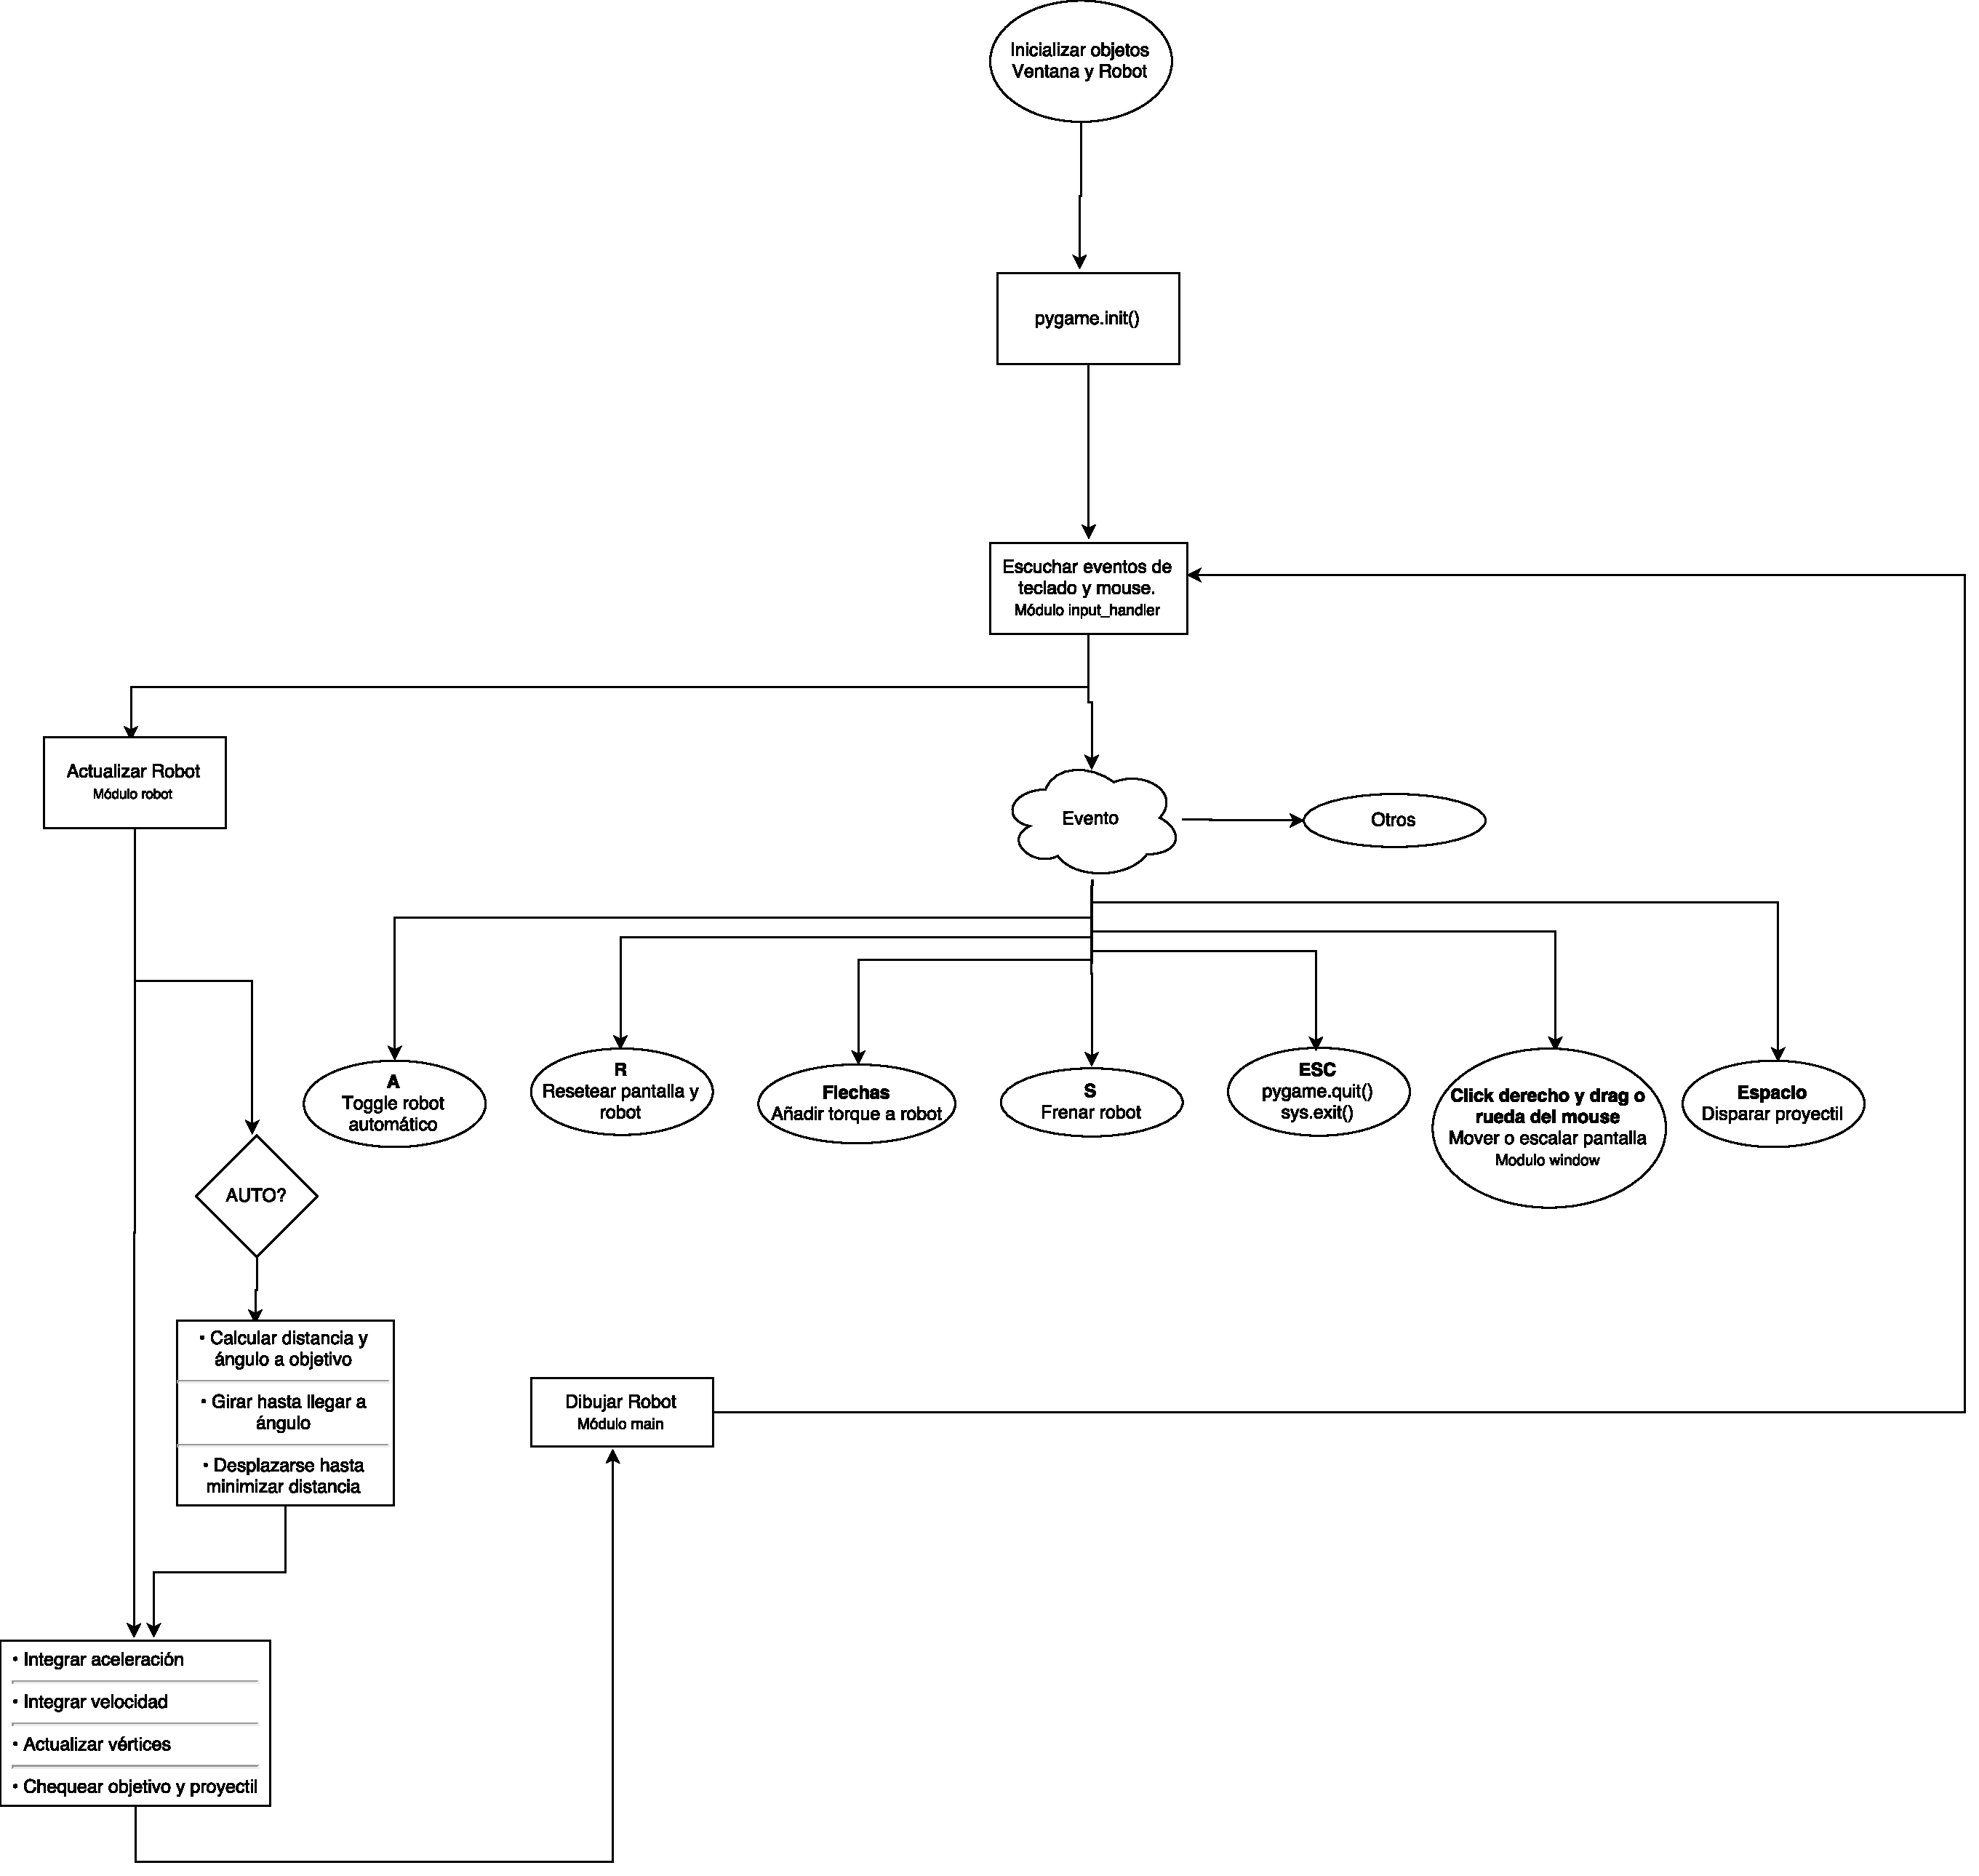
\includepdf[scale=0.8,pagecommand={\captionof{figure}{Diagrama de flujo simplificado}}]{diagram.pdf}

En este caso se vi\'o innecesaria la implementaci\'on de un controlador PD, pues las funciones de control descritas caracterizan completamente el sistema din\'amico implementado, y la \'unica variable que efectivamente afecta la exactitud de la trayectoria es el margen de error aceptable para decir que una maniobra ha finalizado.

Sin embargo, en casos de control reales es imperativo poseer un controlador propiamente tal, pues ninguna cantidad de matem\'atica (por lo menos para sistemas incrustados como Arduino) puede caracterizar todas las posibles variaciones en roce con el suelo, arrastre atmosf\'erico, deslices, variaciones en los motores, etc.

\printbibliography

\end{document}